\documentclass[12pt]{article}

\usepackage{fontspec}
\usepackage{amsmath, amssymb, amsfonts}
\usepackage{graphicx}
\usepackage{hyperref}
\usepackage{color}
\usepackage{geometry}
\geometry{a4paper}

\usepackage{tikz}
\usetikzlibrary{calc, positioning}

\begin{document}
	\begin{minipage}[t]{.5\textwidth}
		{\large Prénom :\\
		Nom :}
	\end{minipage}%
	\begin{minipage}[t]{.5\textwidth}
		\begin{flushright}
			{\Large /30}
		\end{flushright}
	\end{minipage}

	\vspace{3em}
	\begin{center}
			{\Large Examen}\\
			{\large 6e Générale}\\
			14 décembre 2023
	\end{center}
	
	\vspace{3em}
	
	\fbox{\parbox{\linewidth}{%
			\textbf{Consignes :} L'examen commence à 8h10 et se termine à 10h40. Tu as le droit d'avoir une feuille A4 avec les notes que tu auras préparées. Tu peux écrire sur cette feuille ou sur une feuille à part, n'oublie pas de bien écrire tes prénom et nom sur toutes les feuilles que tu utilises. Les machines à calculer sont autorisées. Pose des questions si tu en as besoin. Bon courage !
	}}
	
	\vspace{2em}
	
	\begin{enumerate}
		\item 
			\begin{minipage}[t]{.9\textwidth}
				Résous les calculs vectoriels suivants :
				\begin{enumerate}
					\item $4 \cdot \left(1; -2\right) + 3 \cdot \left(4; 5\right)$
					\item $\left(1; -2; 3\right) - 2 \cdot \left(0; 1; 0\right)$
					\item $\frac{5}{2} \cdot \left(1; 3; -2\right) + \frac{2}{3} \cdot \left(3; 2; -1\right)$
				\end{enumerate}
			\end{minipage}%
			\begin{minipage}{.1\textwidth}
				\begin{flushright}
					{\large /3}
				\end{flushright}
			\end{minipage}
			\vspace{1em}
			
		\item 
			\begin{minipage}[t]{.9\textwidth}
				Calcule graphiquement $\vec{u} - \vec{v}$ :
				\begin{center}
					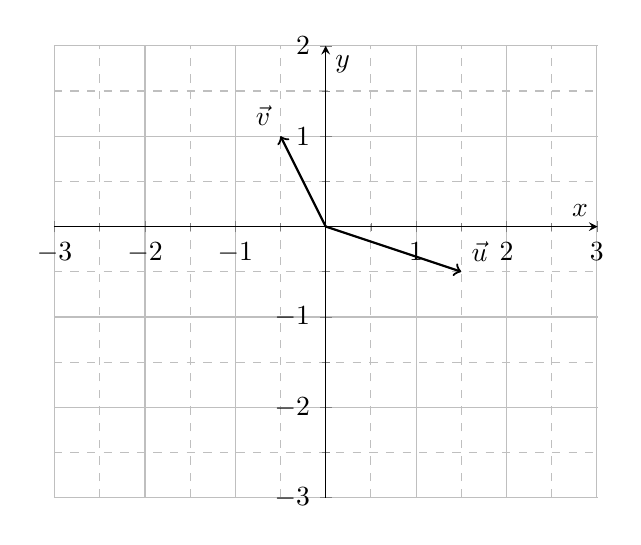
\begin{tikzpicture}
						\begin{axis}[
							width=.7\linewidth,
							axis lines=center,
							xlabel={$x$},
							ylabel={$y$},
							xmin=-3, xmax=3,
							ymin=-3, ymax=2,
							axis equal,
							grid=both,
							minor tick num=1,
							minor grid style={dashed}
							]
							
							\addplot[->, thick] coordinates {(0, 0) (1.5, -0.5)} node[above right] {$\vec{u}$};
							\addplot[->, thick] coordinates {(0, 0) (-0.5, 1)} node[above left] {$\vec{v}$};
						\end{axis}
					\end{tikzpicture}
				\end{center}
			\end{minipage}%
			\begin{minipage}{.1\textwidth}
				\begin{flushright}
					{\large /1}
				\end{flushright}
			\end{minipage}
			\vspace{3em}
			
		\item 
			\begin{minipage}[t]{.9\textwidth}
				Les vecteurs suivants sont-ils colinéaires ? Orthogonaux ? Aucun des deux~?
				\begin{enumerate}
					\item $\left(2; -1; 3\right)$ et $\left(1; 3; \frac{1}{3}\right)$
					\item $\left(1; -1; 1\right)$ et $\left(0; 0; 1\right)$
					\item $\left(1; 2; 3\right)$ et $\left(\frac{1}{2}; 1; \frac{3}{2}\right)$
					\item $\left(1; -1; 4\right)$ et $\vec{0}$
					\item $\left(-1; 2; 3\right)$ et $\left(0; -3; 2\right)$
					\item $\left(1; -1; 3\right)$ et $\left(\frac{-7}{3}; \frac{7}{3}; \frac{-21}{3}\right)$
				\end{enumerate}
			\end{minipage}%
			\begin{minipage}{.1\textwidth}
				\begin{flushright}
					{\large /3}
				\end{flushright}
			\end{minipage}
			\vspace{1em}
			
		\item 
			\begin{minipage}[t]{.9\textwidth}
				Soit les vecteurs $\vec{u} = \left(2; 2; -2\right)$ et $\vec{v} = \left(3; 2; 5\right)$.
				\begin{enumerate}
					\item $\vec{u}$ et $\vec{v}$ sont-ils orthogonaux ?
					\item Soit $\vec{w} = \left(a; 3; b\right)$. Détermine $a$ et $b$ pour que $\vec{w}$ soit orthogonal à $\vec{u}$ et $\vec{v}$.
				\end{enumerate}
			\end{minipage}%
			\begin{minipage}{.1\textwidth}
				\begin{flushright}
					{\large /4}
				\end{flushright}
			\end{minipage}
			\vspace{1em}
			
		\item 
			\begin{minipage}[t]{.9\textwidth}
				Vrai ou faux ? Justifie :
				\begin{enumerate}
					\item Le vecteur $\vec{n}$ est normal au plan $P$ signifie que $\vec{n}$ est un vecteur directeur d'une droite $d$ parallèle au plan $P$.
					\item Si $P \equiv ax + by +cz + d = 0$, alors le vecteur $\vec{n} = \left(a; b; c\right)$ est normal au plan $P$.
					\item Une droite est perpendiculaire à un plan si un vecteur directeur de la droite est un vecteur normal au plan.
					\item Les plans $P_1 \equiv 2x + 3y - z + 2 = 0$ et $P_2 \equiv -6x - 9y + 3z + 1 = 0$ sont parallèles.
				\end{enumerate}
			\end{minipage}%
			\begin{minipage}{.1\textwidth}
				\begin{flushright}
					{\large /4}
				\end{flushright}
			\end{minipage}
			\vspace{1em}
		
		\item 
			\begin{minipage}[t]{.9\textwidth}
				Soit les points $A \equiv \left(1; 2; 1\right)$, $B \equiv \left(3; -1; 2\right)$ et $C \equiv \left(0; 2; -1\right)$. Donne les équations \textit{vectorielle} et \textit{cartésienne} du plan $P$ défini par les points $A$, $B$ et $C$.
			\end{minipage}%
			\begin{minipage}{.1\textwidth}
				\begin{flushright}
					{\large /4}
				\end{flushright}
			\end{minipage}
			\vspace{1em}
		
		\item 
			\begin{minipage}[t]{.9\textwidth}
				Soit le plan $P \equiv 2x - 3y + 4z + 7 = -3$. Donne un vecteur normal du plan $P$.
			\end{minipage}%
			\begin{minipage}{.1\textwidth}
				\begin{flushright}
					{\large /1}
				\end{flushright}
			\end{minipage}
			\vspace{1em}
			
		\item 
			\begin{minipage}[t]{.9\textwidth}
				Soit le plan $P$ d'équation $P \equiv \vec{x} = k_1 \cdot \left(3; -1; 2\right) + k_2 \cdot \left(1; 1; -2\right) + \left(1; 0; -3\right), ~(k_1, k_2 \in \mathbb{R})$. Donne l'équation vectorielle d'un plan $R$ orthogonal à $P$.
			\end{minipage}%
			\begin{minipage}{.1\textwidth}
				\begin{flushright}
					{\large /4}
				\end{flushright}
			\end{minipage}
			\vspace{1em}
			
		\item 
			\begin{minipage}[t]{.9\textwidth}
				Un GPS permet d'obtenir sa position avec trois coordonnées, $x$, $y$ et $z$, exprimées en mètres. Sacha et Alex font une randonnée en montagne et se repèrent avec un GPS. Leurs coordonnées sont les suivantes :
				\begin{itemize}
					\item Sacha : $\left(231; 743; 1782\right)$.
					\item Alex : $\left(-431; 849; 1431\right)$.
				\end{itemize}
			Quelle distance les sépare ?
			\end{minipage}%
			\begin{minipage}{.1\textwidth}
				\begin{flushright}
					{\large /1}
				\end{flushright}
			\end{minipage}
			\vspace{1em}
			
		\item 
			\begin{minipage}[t]{.9\textwidth}
				Soit $P$ un plan d'équation $P \equiv 4x -2y + 3z - 6 = 0$ et le point $A \equiv \left(1; 0; 1\right)$. Donne l'équation vectorielle d'une droite normale à $P$ et passant par le point $A$.
			\end{minipage}%
			\begin{minipage}{.1\textwidth}
				\begin{flushright}
					{\large /1}
				\end{flushright}
			\end{minipage}
			\vspace{1em}
			
		\item 
			\begin{minipage}[t]{.9\textwidth}
				Soit les figures suivantes :
				\begin{itemize}
					\item Le plan $P$ d'équation $P \equiv \vec{x} = k_1 \cdot \left(2; 0; 1\right) + k_2 \cdot \left(1; 1; 3\right) + \left(-2; -2; -1\right), ~(k_1, k_2 \in \mathbb{R})$.
					\item La droite $D$ d'équation $D \equiv \vec{x} = k \cdot \left(a; -2; b\right) + \left(2; 1; -2\right)$.
				\end{itemize}
				Pour quelle valeur des paramètres $a$ et $b$ la droite $D$ sera-t-elle orthogonale au plan $P$ ?
			\end{minipage}%
			\begin{minipage}{.1\textwidth}
				\begin{flushright}
					{\large /4}
				\end{flushright}
			\end{minipage}
			
	\end{enumerate}
	
\end{document}